\documentclass[../main.tex]{subfiles}
\graphicspath{{../images/}}

\begin{document}
\subsection*{Lecture 12: \hfill  2/16/24}
\hrule \vspace{10px}
\section{Lagrange's Equations}

From last time: we defined the path
\begin{align*}
    S = \int_a^b f(x, y(x), y'(x)) \dd x
\end{align*}
Goal: find $y(x)$ that minimizes $S$ using EL
\begin{align*}
    \text{EL:} \quad \pdv{f}{y} - \dv{x}(\pdv{f}{y'}) = 0
\end{align*}
where near the minimum $\delta S = 0$. From the EL, $y(x)$ is a stationary point of $S$(could also
be a maximum!). 

\paragraph*{Lagrangian} In Classical Mechanics, we use a specific form 
\begin{align*}
    \mathcal{L} = T - V
\end{align*}
this has the units of energy and the action $S$ has the units $[S] = [E \cdot T]$ similar to
planck's constant $\hbar$.
\paragraph*{3D Cartesian} $x, y, z = q_1, q_2, q_3$
\begin{align*}
    T &= \frac{1}{2} m v^2 = \frac{1}{2} m (\dot x^2 + \dot y^2 + \dot z^2) \\
    U &= U(x, y, z)
\end{align*}
where the potential energy only depends on the position and $T$ only depends on the velocity, so 
\begin{align*} 
    \mathcal{L} = \frac{1}{2} m (\dot x^2 + \dot y^2 + \dot z^2) - U(x, y, z)
\end{align*}
and the EL equation for the Lagrangian is
\begin{align*}
    \pdv{\mathcal{L}}{q_i} = \dv{t} \pdv{\mathcal{L}}{\dot q_i}
\end{align*}
For the 3D case, we have 3 equations of motion: For $x$ we have 
\begin{align*}
    \pdv{\mathcal{L}}{x} = - \pdv{U}{x}, \quad \pdv{\mathcal{L}}{\dot x} = m \dot x
\end{align*}
and using the EL equation, we get
\begin{align*}
    -\pdv{U}{x} = \dv{t}(m \dot x) = m \ddot x
\end{align*}
which is Newton's second law $F_x = m a_x$ where $\vb{F} = - \grad U$. We can now get the general form
\begin{align*}
    \vb F = m \vb a
\end{align*}
\paragraph*{Polar Coordinates} $q: (r, \phi)$ we know that
\begin{align*}
    \vb v = v_r \vu r + v_\phi \vu* \phi = \dot r \vu r + r \dot \phi \vu* \phi
\end{align*}
and
\begin{align*}
    U = U(r, \phi), \qquad T = \frac{1}{2} m v^2 = \frac{1}{2} m (\dot r^2 + r^2 \dot \phi^2)
\end{align*}
first we find the parts EL equation for $r$
\begin{align*}
    \pdv{\lagr}{r} &= mr \dot \phi^2 - \pdv{U}{r} \\
    \pdv{\lagr}{\dot r} &= m \dot r
\end{align*}
and the EL equation is
\begin{align*}
    mr \dot \phi^2 - \pdv{U}{r} = \dv{t}(m \dot r) \\
    m(\ddot r - r \dot \phi^2) = - \pdv{U}{r}
\end{align*}
which gives us N2L for $r$. For $\phi$ we have
\begin{align*}
    \pdv{\lagr}{\phi} &= -\pdv{U}{\phi} \\
    \pdv{\lagr}{\dot \phi} &= m r^2 \dot \phi
\end{align*}
and from the EL equation we get
\begin{align*}
    -\pdv{U}{\phi} = \dv{t}(mr^2 \dot \phi ) = m(2 r \dot r \dot \phi + r^2 \ddot \phi)
\end{align*}
dividing both sides by $r$
\begin{align*}
    -\frac{1}{r} \pdv{U}{\phi} = m(r \ddot \phi + 2 \dot r \dot \phi) = -(\grad U)_\phi
\end{align*}
from both forms we know that the two parts of the EL represent the momentum and force:
\begin{align*}
    \pdv{\lagr}{\dot q_i} &= p_i \qqtext{generalized momentum} \\
    \pdv{\lagr}{q_i} &= F_i \qqtext{generalized force} 
\end{align*}
where $F_i = \dv{t} p_i$ is the generalized N2L.
\paragraph*{Example:}  Mass $m$ sliding down a frictionless \emph{moving} ramp $M$. First we choose the
coordinates $x$ moving along withe the ramp and $y$ down in the perpendicular direction. For the
ramp $M$:
\begin{align*}
    T_M = \frac{1}{2} M \dot q_2^2, \quad U_M = 0
\end{align*}
and for the mass $m$: First we decompose the velocity of $m$ into the $x$ and $y$ components
\begin{align*}
    \vb v_m = \dot x \vu x + \dot y \vu y = \vu y(\dot q_1 \sin \alpha)
        + \vu x(\dot q_1 \cos \alpha + \dot q_2)
\end{align*}
and the kinetic and potential energies are
\begin{align*}
    T_m = \frac{1}{2} m v_m^2 = \frac{1}{2} m (\dot q_1^2 + 2 \dot q_1 \dot q_2 \cos \alpha + \dot q_2^2) \\
    U_m = mgy = -mg (\dot q_1 \sin \alpha)
\end{align*}
using the Lagrangian $\mathcal{L} = T - U = T_M + T_m - U_M - U_m$ we get
\begin{align*}
    \pdv{\lagr}{q_2} &= 0, \quad \pdv{\lagr}{\dot q_2} = M \dot q_2 + m \dot q_2 + m \dot q_1 \cos \alpha
\end{align*}
and the EL equation gives us
\begin{align*}
    (M + m) \ddot q_2 + m \ddot q_1 \cos \alpha = 0 \\
    a_2 = \ddot q_2 = -\frac{m \ddot q_1 \cos \alpha}{M + m}
\end{align*}
and for $q_1$ we have
\begin{align*}
    \pdv{\lagr}{q_1} &= mg \sin \alpha,
        \quad \pdv{\lagr}{\dot q_1} = m (\dot q_1 + \dot q_2 \cos \alpha)
\end{align*}
and the EL equation gives us
\begin{align*}
    mg \sin \alpha = m (\ddot q_1 + \ddot q_2 \cos \alpha)
\end{align*}
and since we have two equations and two unknowns, we can solve for $\ddot q_1$ and $\ddot q_2$.
\begin{align*}
    \ddot q_1 = \frac{g \sin \alpha}{1 - \frac{m\cos^2 \alpha}{m + M}} = const \\
    \ddot q_2 = -\frac{m \ddot q_1 \cos \alpha}{M + m} = const
\end{align*}
for $\alpha = 90^\circ$, we get $\ddot q_1 = g$ and $\ddot q_2 = 0$ which is the same as a free falling.
For and infinitely heavy ramp $M \to \infty$, we get $\ddot q_1 = g \sin\alpha$. For $M \to 0$ we
get $\ddot q_1 = g / \sin\alpha$ which doesn't make sense because the force on the mass would be
infinite. The normal force $N \to 0$ as $M \to 0$ and the mass would be in free fall.

\newpage
\subsection*{Lecture 13: \hfill 2/19/24}
\hrule \vspace{10px}

\paragraph*{Review} Lagrangian: For a general integral
\begin{align*}
    S \int f(x,y, y') \dd x
\end{align*}
find $y(x)$ minimizing $S$ using the EL equation
\begin{align*}
    \pdv{f}{y} = \dv{x}(\pdv{f}{y'})
\end{align*}
For Classical Mechanics, we use the Lagrangian in the generalized coordinate system $q_i$ we define
the action $S$ as
\begin{align*}
    S = \int \lagr (q_i, \dot q_i, t) \dd t \qqtext{find} q(t)
\end{align*}
and from the EL equation we get
\begin{align*}
    \pdv{\lagr}{q_i} = \dv{t} \pdv{\lagr}{\dot q_i}
\end{align*}
for each degree of freedom. We define the Lagrangian in CM as the quantity $\lagr = T - U$

\paragraph*{Examples, Examples, and more Examples:} A pendulum but its spining on its axis. We 
first find  the energies:
\begin{figure}[ht]
    \centering
    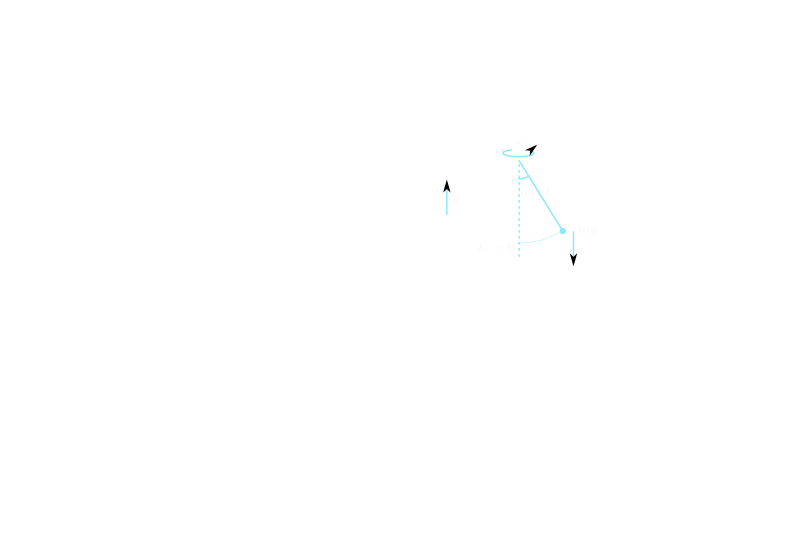
\includegraphics[width=0.5\textwidth]{spinningpendulum.png}
    \caption{Pendulum}
\end{figure}
\begin{align*}
    T &= \frac{1}{2} m v^2 = \frac{1}{2} m ((\omega L \sin \theta)^2 + (L \dot \theta)^2) \\
    U &= mg y = mg L (1 - \cos \theta)
\end{align*}
from EL equation we get
\begin{align*}
    \pdv{\lagr}{\theta} &= \frac{1}{2} m\omega^2 L^2 (2 \sin\theta \cos\theta) - mg L \sin\theta 
        = m\omega^2 L^2 \cos \theta \sin \theta - mgL \sin\theta \\
    \pdv{\lagr}{\dot \theta} &= m L^2 \dot \theta \\
    \dv{t} \pdv{\lagr}{\dot \theta} &= m L^2 \ddot \theta
\end{align*}
so 
\begin{align*}
    m L^2 \ddot \theta &= m\omega^2 L^2 \cos \theta \sin \theta - mgL \sin\theta \\
    \ddot \theta &= \omega^2 \cos \theta \sin \theta - \frac{g}{L} \sin \theta
\end{align*}
when $\omega = 0$ we get the simple pendulum $\ddot \theta = - \frac{g}{L} \sin \theta$. Identifying
the the equilibrium points where $\ddot \theta = 0 \implies$
\begin{align*}
    \sin \theta = 0 \implies \theta = 0, \pi
\end{align*}
at $\theta = 0$ the pendulum is just hanging vertically down which we can physically deduce as a
stable equilibrium point. To check this analytically we can assume a small deviation from the
equilibrium point:
\begin{align*}
    \theta &= 0 + \epsilon \\
    \cos(0 + \epsilon) &= 1 - \frac{\epsilon^2}{2} \approx 1 \\
    \sin(0 + \epsilon) &= \epsilon - \frac{\epsilon^3}{6} \approx \epsilon \\
\end{align*}
and we get
\begin{align*}
    \ddot \theta &= (\omega^2 - \frac{g}{L}) \theta \\
    \ddot \theta &= - \Omega^2 \theta \implies \mathrm{Stable} \\
    \ddot \theta &= \Omega^2 \theta \implies \mathrm{Unstable}
\end{align*}
where 
\begin{align*}
    \omega^2 < \frac{g}{L} \implies \mathrm{Stable} \\
    \omega^2 > \frac{g}{L} \implies \mathrm{Unstable}
\end{align*}
when they are equal $\omega^2 = \frac{g}{L}$ we get a simple pendulum. Finding another equilibrium
point at
\begin{align*}
    \omega^2 \cos\theta - \frac{g}{L} &= 0 \\
    \cos\theta &= \frac{g}{L\omega^2}, \qquad \theta = \pm \arccos(\frac{g}{L\omega^2})
\end{align*}
where there only exists a solution when
\begin{align*}
    \omega^2 > \frac{g}{L}
\end{align*}
since $\cos\theta \leq 1$. For this case, we can also look at the radial force in polar:
\begin{align*}
    F_r = m\ddot r - mr \omega^2
    \qor m\ddot r = F_r + mr \omega^2
\end{align*}
where in the second equation we can see that the sum of the centrifugal force and $F_r$ sums to zero
so
\begin{align*}
    \tan \theta = \frac{F_r}{mg} = \frac{mL \sin\theta\omega^2}{mg} \\
    \implies \frac{L\omega^2}{g} = \frac{1}{\cos\theta} \\
    \cos\theta = \frac{g}{L\omega^2}
\end{align*}
from the force analysis we can see that the centrifugal force is balanced by the radial force.
Substituing the equilibium position back into the EOM 
\begin{align*}
    \cos\theta_o = \frac{g}{L\omega^2} \to \theta = \theta_o + \epsilon
\end{align*}
Using Taylor Expansion, $f(x) = f(x_o) + f'(x_o) (x-x_o)$, the sine and cosine terms are
\begin{align*}
    \cos\theta &= \cos(\theta_o + \epsilon) = \cos\theta_o - \sin\theta_o \epsilon \\
    \sin\theta &= \sin(\theta_o + \epsilon) = \sin\theta_o + \cos\theta_o \epsilon
\end{align*}
so the EOM becomes
\begin{align*}
    \ddot \theta = (- \omega^2 \sin\theta_o \epsilon) (\sin\theta_o + \cos\theta_o \epsilon) \\
    \ddot \epsilon = -\omega^2 \sin^2(\theta_o) \epsilon
\end{align*}
where we have Bifurcation at $\omega^2 = \frac{g}{L}$. We can see that the EOM for $\epsilon$ is
similar to the harmonic oscillator so:
\begin{align*}
    \epsilon = A \cos(\Omega t - \delta) \qquad \Omega = \omega \sin\theta_o
\end{align*}
\paragraph*{HW 5} Given $f(x, y, y')$. Independence of $y$ means:
\begin{align*}
    f(x, y') \implies \pdv{f}{y'} = constant \\
    \lagr(t, \dot q) \implies \pdv{\lagr}{\dot q} = constant
\end{align*}
so for the Lagrangian
\begin{align*}
    \lagr &= T - U = \frac{1}{2} m \dot x^2 - U(x) \qquad \pdv{\lagr}{q_i} = F_i \qqtext{generalized force} \\
    \pdv{\lagr}{\dot x} &= m \dot x = conserved, \quad \pdv{U}{x} = 0
\end{align*}
if $\lagr$ doesn't depend on $x$, then $p_x$ (momentum) is conserved. So for the generalized 
Lagrangian
\begin{align*}
    \lagr(q_1, \dots, q_n, \dot q_1, \dots, \dot q_n, t) \\
    \mathrm{If} \quad \pdv{\lagr}{q_i} = 0, \quad  \pdv{\lagr}{\dot q_i} = \mathrm{conserved}
\end{align*}
So symmetry $\implies$ conservation (Noether's Theorem).

\newpage
\subsection*{Lecture 14: \hfill 2/21/24}
\hrule \vspace{10px}

\paragraph*{Conservation} The two types: 
\begin{itemize}
    \item If $f(x, y')$ is independent of $y$, then
    \begin{align*}
        \pdv{f}{y'} = \text{constant over } x
    \end{align*}
    or if $\lagr$ is independent of $q_i$, then
    \begin{align*}
        \pdv{\lagr}{q_i} = \text{constant over } t = p_i
    \end{align*}
    \item If $f(y, y')$ is independent of $x$, then
    \begin{align*}
        f - y' \pdv{f}{y'} = \text{constant over } x
    \end{align*}
    or if $\lagr$ is independent of $t$, then
    \begin{align*}
        \lagr - \dot q_i \pdv{\lagr}{\dot q_i} = \text{constant over } t
    \end{align*}
\end{itemize}
looking at this more closely:
    \begin{align*}
        \lagr &= T - U = \frac{1}{2} m \dot q^2 - U(q)
    \end{align*}
    where
    \begin{align*}
        \dot q \pdv{\lagr}{\dot q} &= m \dot q^2; \\
        \dot q \pdv{\lagr}{\dot q} - \lagr &= m \dot q^2 - \frac{1}{2} m \dot q^2 + U \\
        &= \frac{1}{2} m \dot q^2 + U = T + U = E
    \end{align*}
    this is this Hamiltonian 
    \begin{align*}
        \sum_i p_i \dot q_i - \lagr = \mathcal H = E
    \end{align*}
\paragraph*{Noether's Theorem} For a system independent of $t \leftrightarrow$ the system has
time-translation symmetry

$\implies$ conservation of energy

\paragraph*{Dependence on $t$} $U = U(q, t)$ e.g. Mass of sun is increasing over time, the potential
energy is dependent on time, so the system is not conservative. 

\paragraph*{Pendulum thoughts:} In our pendulum example, we chose $q = \theta$, but we could also
choose $q_1 = x$ and $q_2 = y$. The truth lies in the fact that we intuitively chose $q_1 = r$ and
$q_2 = \theta$. So in transforming from Cartesian coordinates
\begin{align*}
    x = r\cos\theta, \qquad y = r\sin\theta, \qquad r = L
\end{align*}
where we have a `constraint' $r = L$\dots

\paragraph*{Legal Terms: Formal Definition of Constraints} In the beginning, we defined the first defined position with
\begin{align*}
    \vb r = (x, y, z)
\end{align*}
for the generalized coordinates we have
\begin{align*}
    \vb r = \vb r(q_1, \dots, q_n, t)
\end{align*}
where we decided that in a 3D system $n = 3$. A constraint is an equation
\begin{align*}
    f(q_1, \dots, q_n) = 0
\end{align*}
where this is a \emph{holonomic} (whole) constraint and to find the number of generalized coordinates:
\begin{align*}
    \text{\# of generalized coordinates we need} &= \text{\# of dimensions} - \text{\# of constraints}  \\
    &= \text{\# of degrees of freedom}
\end{align*}
this is only true for holonomic constraints. For \emph{nonholonomic} constraints, it is more complicated
e.g. A ball on a horizontal table: We can see that \# of generalized coordinates = 2, but to
describe the position of the ball i.e. a dot on the ball, we need 3 more coordinates (Euler angles).
So the configuration of the ball is described by 5 coordinates $(x, y, \alpha, \beta, \gamma)$. In
other words, the configuration is path dependent and we see a nonholonomic constraint.

\paragraph*{Example:} What are the constraints for the mass sliding down a moving mass? The 
holonomic constraints are the vertical position of the ramp $y_M = 0$, and from $x_m, y_m, x_M$ we 
know the $x_{COM} =$ constant.

\paragraph*{Fact!} A constraint is enforced by a constraint force $\vb F_c \perp$ path(in the
pendulum example, the normal force $N$). Finding this force where $f(q_i) = 0$ can be found by
taking the gradient of the function $\grad f$. So
\begin{align*}
    \vb F_c = \lambda \grad f
\end{align*}

\newpage
\subsection*{Lecture 15: \hfill 2/23/24}
\hrule \vspace{10px}
\paragraph*{Review}
\begin{itemize}
    \item Convservation: Lagrangian is independent of time $\implies$ conservation of energy
\end{itemize}

\paragraph*{Lagrange Multiplier} Want to find $q_i(t)$ by minimizing
$S = \int \lagr(q_i, \dot q_i, t) \dd t$.
\paragraph*{} $\star$ Under holonomic constraints,
\begin{align*}
    f(q_i) = 0
\end{align*}
So we introduce a new unknown $\lambda(t)$ and the new minimizing integral becomes
\begin{align*}
    I = \int (\lagr - \lambda f) \dd t
\end{align*}
The EL eqn for $\lambda(t):\quad f=0$
\begin{align*}
    \pdv{(\lagr - \lambda f)}{\lambda} = -f \qquad \pdv{(\lagr - \lambda f)}{\dot \lambda} = 0
\end{align*}
The EL eqn for $q_i(t)$:
\begin{align*}
    F_i = \pdv{(\lagr - \lambda f)}{q_i} = \dv{t} \pdv{(\lagr - \lambda f)}{\dot q_i}
\end{align*}
or
\begin{align*}
    F_i = \pdv{\lagr}{q_i} - \lambda \pdv{f}{q_i} \qqtext{where} \pdv{\lagr}{q_i} = p_i
\end{align*}
So we are given $N+1$ unknowns and $N+1$ EL eqns with the addition of the lagrange multiplier.
\paragraph*{Simple Pendulum (revisited)} We have the Lagrangian
$\lagr(x, y, \dot x, \dot y) = T - U$ where 
\begin{align*}
    T &= \frac{1}{2} m (\dot x^2 + \dot y^2) \\
    U &= -mgy
\end{align*}
so
\begin{align*}
    \lagr = \frac{1}{2} m (\dot x^2 + \dot y^2) + mgy
\end{align*}
and using the constraint of the fixed length; $f(x, y) = x^2 + y^2 - L^2 = 0$ we get
\begin{align*}
    \ell = \lagr - \lambda f = \frac{1}{2} m (\dot x^2 + \dot y^2) + mgy - \lambda(x^2 + y^2 - L^2)
\end{align*}
and the EL eqns are
\begin{itemize}
    \item $x$:
    \begin{align*}
        -2\lambda x = m \ddot x
    \end{align*}
    \item $y$:
    \begin{align*}
        mg - 2\lambda y = m \ddot y
    \end{align*}
    \item $\lambda$: Left as an exercise
\end{itemize}
We can see from force analysis of the pendulum:
\begin{align*}
    m\ddot x = F_x = -2\lambda x \qquad m\ddot y = F_y = mg - 2\lambda y
\end{align*}
so the lagrange multiplier quantities are equivalent to the tension
\begin{align*}
    T_x = 2\lambda x \qquad T_y = 2\lambda y
\end{align*}
where the negative sign indicates the correct direction of Tension.

\paragraph*{Pendulum in Polar} $(r, \phi)$
\begin{align*}
    \lagr(r, \phi, \dot r, \dot \phi) = \frac{1}{2} m (\dot r^2 + r^2 \dot \phi^2) - mgr\cos\theta
\end{align*}
where
\begin{align*}
    f = r - L = 0
\end{align*}
so we get the EL eqns
\begin{align*}
    -\lambda + mg\cos\theta = m\ddot r \qquad \lambda = mg\cos\theta
\end{align*}

\paragraph*{Use cases of Lagrange Multipliers} Although the previous example seems trivial, we 
consider its use in the example of a heavy chain hanging from two poles: The linear mass density is
given by
\begin{align*}
    M = \rho L
\end{align*}
to find the shape, we need to minimize the potential energy
\begin{align*}
    S = \int \dd m g y
\end{align*}
where $\dd m = \rho \dd s$ is the mass of a segment and under the constraint of chain length:
\begin{align*}
    L = \int \dd s = \int \dd x \sqrt{1 + y'^2} 
\end{align*}
so
\begin{align*}
    S = \int \rho gy \sqrt{1 + y'^2} \dd x
\end{align*}
and introducing $\lambda$ we minimize
\begin{align*}
    \int (\rho g y - \lambda) \sqrt{1 + y'^2} \dd x = S - \lambda L
\end{align*}
we can see that it is independent of $x$ so
\begin{align*}
    f = (\rho g y - \lambda) \sqrt{1 + y'^2}
\end{align*}
and
\begin{align*}
    f - y' \pdv{f}{y'} = \text{constant} = C
\end{align*}
so the EL eqn is:
\begin{align*}
    \pdv{f}{y'} = (\rho g y - \lambda) \frac{y'}{\sqrt{1 + y'^2}}
\end{align*}
and therefore
\begin{align*}
    f - y' \pdv{f}{y'} = (\rho g y - \lambda)
        \qt[\sqrt{1 + y'^2} - \frac{y'^2}{\sqrt{1 + y'^2}}] = \text{constant}
\end{align*}
and quantity in brackets is
\begin{align*}
    [\;] = \frac{1}{\sqrt{1 + y'^2}}
\end{align*}
so
\begin{align*}
    \qt(\frac{\rho g y - \lambda}{\sqrt{1 + y'^2}})^2 &= C^2 \\
    1 + y'^2 &= \frac{(\rho g y - \lambda)^2}{C^2}
\end{align*}
for an easier solution we choose a change of variables
\begin{align*}
    \tilde y = \frac{\rho g y - \lambda}{C} \implies \tilde y' = \frac{\rho g}{C} y'
\end{align*}
and redifining the $x$
\begin{align*}
    \tilde y'^2 = 1 + y'^2
    \begin{cases}
        \tilde x = \frac{\rho g}{C} x \\
        \dv{\tilde y}{\tilde x} = \dv{y}{x}
    \end{cases}
\end{align*}
and we get
\begin{align*}
    \tilde y = \pm \cosh(\tilde x - \tilde x_0)
\end{align*}
we could have also used the Lagrange Multiplier for the Maximum Area Fixed Perimeter problem.
\end{document}